% !TeX root = ../../thesis.tex

\section{Pseudorandom Noise Sequences}
\label{sec:pn-sequences}

PN sequences are sequences which look like they are randomly generated but they are easily generated in software or hardware.
They are generated with linear shift registers of length $n$.
The sequences have the following noise-like properties~\cite{mitra2008pseudo}:

\begin{itemize}
	\item Balance property:	Any PN sequence of length $L = 2^n - 1$ contains exactly $2^{n-1}$ ones and exactly $2^{n-1} - 1$ zeros.

	\item Runs property: A run is a subset of the sequence where all the consecutive numbers are the same. In any PN sequence, $1/2$ of the runs have length 1, $1/4$ have length 2, $1/8$ have length 3 and so on.

	\item Autocorrelation property: The autocorrelation function of a PN sequence will take on two values as can be seen in \autoref{eq:autocorr-pn} and \autoref{fig:autocorr-pn}.


\end{itemize}

\begin{equation}
	\label{eq:autocorr-pn}
	R(\tau) = 
		\begin{cases}
			L    & \quad \text{if } \tau = 0 \\
			-1   & \quad \text{if } \tau \neq 0 \\
		\end{cases}
\end{equation}

\begin{figure}[h]
	\centering
	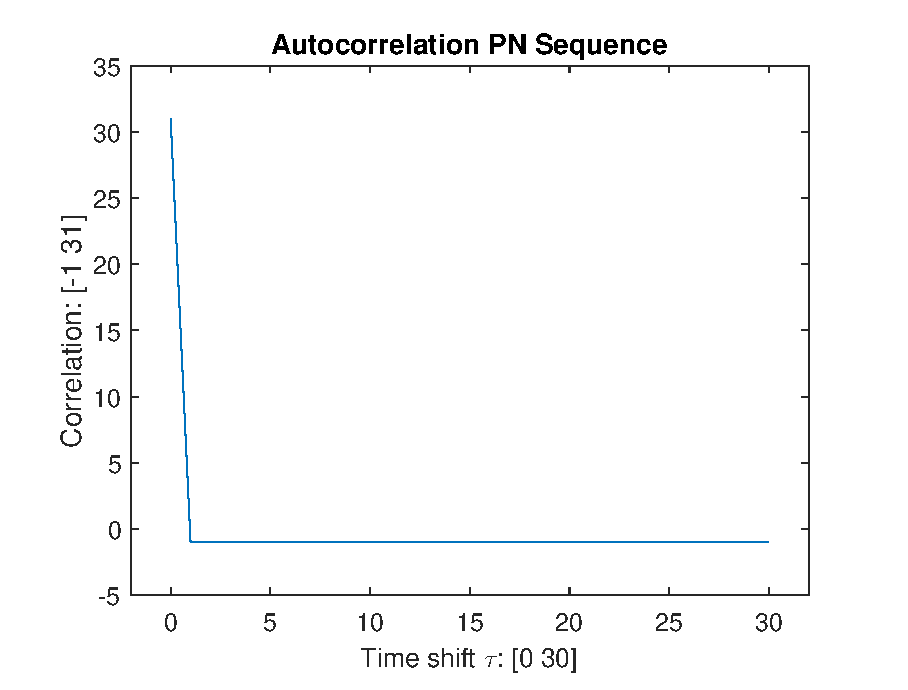
\includegraphics[width=\textwidth]{chapters/cdma-chapters/autocorr-pn.eps}
	\caption{Autocorrelation of PN sequence of length 31.}
	\label{fig:autocorr-pn}
\end{figure}

PN sequences are generated using a linear feedback shift register (LFSR) \cite{Wang:1988:LFS:52007.52024}.
\autoref{fig:lfsr} shows an $n$ length LFSR with some XOR gates attached to it.
The LFSR is defined entirely by the feedback function, also called a characteristic polynomial.
It determines the length and the type of sequence generated.
The polynomial looks like \autoref{eq:lfsr-polynomial}.

\begin{equation}
	\label{eq:lfsr-polynomial}
	p(x) = x^n + C_{n-1} x^{n-1}  + C_{n-2} x^{n-2} + \dotsc + C_{2} x^{2}  + C_{1} x  + C_{0}
\end{equation}

\begin{figure}[h]
	\centering
	\begin{tikzpicture}


		\node[block                  ] (last_register) {$s_{n-1}$};
		\node[block, right = 1cm of last_register] (second_last_register) {$s_{n-2}$};
		\draw[line] (last_register.east) -- (second_last_register.west) ;

		\node[block, right = 3cm of second_last_register] (second_register) {$s_{1}$};
		\node[block, right = 1cm of second_register] (mid_register) {$s_{0}$};
		\draw[line] (second_register.east) -- (mid_register.west) ;

		\draw[dashed, line] (second_last_register.east) -- (second_register.west) ;

		\node[coordinate, right = 2cm of mid_register] (output_point) {};
		\draw[line] (mid_register.east) -- (output_point.west) node [midway, above] {output};

		\node[XOR, scale=2, below = 2cm of second_register] (first_xor) {};
		\draw[line] (second_register.south) -- (first_xor.north) node [midway, right] {$C_1$};
		\draw[line] (mid_register.south) |- (first_xor.east) node [pos=0.21, right] {$C_0$};

		\node[coordinate, right = 1.5cm of second_last_register] (h) {};
		\node[XOR, scale=2, below = 2.5cm of h] (mid_xor) {};
		\draw[line] (first_xor.west) -- (mid_xor.east) ;
		\draw[dashed, line] (h.south) -- (mid_xor.north) ;

		\node[XOR, scale=2, below = 2cm of second_last_register] (second_last_xor) {};
		\node[XOR, scale=2, below = 2cm of last_register] (last_xor) {};

		\draw[line] (second_last_register.south) -- (second_last_xor.north) node [midway, right] {$C_{n-2}$};
		\draw[line] (mid_xor.west) -- (second_last_xor.east) ;
		
		\draw[line] (second_last_xor.west) -- (last_xor.east) ;
		\draw[line] (last_register.south) -- (last_xor.north) node [midway, right] {$C_{n-1}$};

		\node[coordinate, left = 1cm of last_register] (return_point) {};
		
		\draw[line] (last_xor.west) -| (return_point) -- (last_register.west) ;




	\end{tikzpicture}
	\caption{Linear feedback shifter register of length $n$, with XOR gates.}
	\label{fig:lfsr}
\end{figure}


For PN sequences, there exists no formula for the cross-correlation of two different PN sequences. 
Exhaustive analysis is required to find out which sequences or entire sets have the cross-correlation characteristics that are good enough for the user's application.

The size of the code set is limited.
For a LFSR with $n$ registers, the maximum number of possible codes $C$ is given by \autoref{eq:num-of-pn-codes} \cite{mutagi1996pseudo}, where $P_i$ are the prime factors of $2^n - 1$ and $\alpha_i$ is the power of $i$th prime factor.

\begin{equation}
	\label{eq:num-of-pn-codes}
	C = \frac{1}{n} \prod \{ P_{i} ^ {(\alpha_i - 1)} \times (P_i - 1) \}
\end{equation}

For example when using a LFSR of size $n = 6$, $2^n - 1 = 63$, which can be factored into $3^2 \times 7$.
Giving $P_1 = 3$, $P_2 = 7$, $\alpha_1 = 2$ and $\alpha_2 = 1$.
Thus, the maximum number of codes is: $C = \frac{1}{6} \times \{ 3^{2 - 1} \times (3 - 1) \} \times \{ 7^{1 - 1} \times (7 - 1) \} = 6$.
Another example: Say there are going to be 144 user, so 144 codes are needed. 
This means a code length of 4095 chips.
















\subsection{Gold Sequences}
\label{subsec:gold-sequences}

Gold sequences are a type of PN sequence. 
They are created by using two LFS registers as shown in \autoref{fig:gold-lfsr}.
In this figure there are two vectors $s$ and $t$ and two polynomials $C$ and $D$.
For a sequence to be constructed in this way that is a Gold sequence, only preferred pairs of polynomials can be used \cite{kedia2012comparative}.
When we have the polynomials $p(x)$ and $q(x)$, which are a preferred pair and produces the PN sequences $d_1$ and $d_2$ respectively, the resulting set of Gold codes is defined as can be seen in \autoref{eq:gold-def}, where $T^n$ represent the cyclic shift of $n$ bits.

\begin{equation}
	\label{eq:gold-def}
	Gold(d_1, d_2) = \{ d_1, d_2, d_1 \oplus d_2, d_1 \oplus Td_2, d_1 \oplus T^2d_2, \dotsc, d_1 \oplus T^{L - 1}d_2 \}
\end{equation}


\begin{figure}[h]
	\centering
	\begin{tikzpicture}

		\node[block                  ] (last_register1) {$s_{n-1}$};
		\node[block, right = 1cm of last_register1] (second_last_register1) {$s_{n-2}$};
		\draw[line] (last_register1.east) -- (second_last_register1.west) ;

		\node[block, right = 3cm of second_last_register1] (second_register1) {$s_{1}$};
		\node[block, right = 1cm of second_register1] (mid_register1) {$s_{0}$};
		\draw[line] (second_register1.east) -- (mid_register1.west) ;

		\draw[dashed, line] (second_last_register1.east) -- (second_register1.west) ;

		\node[coordinate, right = 1cm of mid_register1] (output_point1) {};

		\node[XOR, scale=2, above = 2cm of second_register1] (first_xor1) {};
		\draw[line] (second_register1.north) -- (first_xor1.south) node [midway, right] {$C_1$};
		\draw[line] (mid_register1.north) |- (first_xor1.east) node [pos=0.21, right] {$C_0$};

		\node[coordinate, right = 1.5cm of second_last_register1] (h1) {};
		\node[XOR, scale=2, above = 2.5cm of h1] (mid_xor1) {};
		\draw[line] (first_xor1.west) -- (mid_xor1.east) ;
		\draw[dashed, line] (h1.north) -- (mid_xor1.south) ;

		\node[XOR, scale=2, above = 2cm of second_last_register1] (second_last_xor1) {};
		\node[XOR, scale=2, above = 2cm of last_register1] (last_xor1) {};

		\draw[line] (second_last_register1.north) -- (second_last_xor1.south) node [midway, right] {$C_{n-2}$};
		\draw[line] (mid_xor1.west) -- (second_last_xor1.east) ;
		
		\draw[line] (second_last_xor1.west) -- (last_xor1.east) ;
		\draw[line] (last_register1.north) -- (last_xor1.south) node [midway, right] {$C_{n-1}$};

		\node[coordinate, left = 1cm of last_register1] (return_point1) {};
		
		\draw[line] (last_xor1.west) -| (return_point1) -- (last_register1.west) ;

		%%%%%%%%%%%%%%%%%%%%%%%%%%%%%%%%%%%%%%%%%%%%%%%%%%%%%%%%%%%%%%%%%%%%%%%%%%%%


		\node[block, below = 2cm of last_register1] (last_register) {$t_{n-1}$};
		\node[block, right = 1cm of last_register] (second_last_register) {$t_{n-2}$};
		\draw[line] (last_register.east) -- (second_last_register.west) ;

		\node[block, right = 3cm of second_last_register] (second_register) {$t_{1}$};
		\node[block, right = 1cm of second_register] (mid_register) {$t_{0}$};
		\draw[line] (second_register.east) -- (mid_register.west) ;

		\draw[dashed, line] (second_last_register.east) -- (second_register.west) ;

		\node[coordinate, right = 1cm of mid_register] (output_point) {};

		\node[XOR, scale=2, below = 2cm of second_register] (first_xor) {};
		\draw[line] (second_register.south) -- (first_xor.north) node [midway, right] {$D_1$};
		\draw[line] (mid_register.south) |- (first_xor.east) node [pos=0.21, right] {$D_0$};

		\node[coordinate, right = 1.5cm of second_last_register] (h) {};
		\node[XOR, scale=2, below = 2.5cm of h] (mid_xor) {};
		\draw[line] (first_xor.west) -- (mid_xor.east) ;
		\draw[dashed, line] (h.south) -- (mid_xor.north) ;

		\node[XOR, scale=2, below = 2cm of second_last_register] (second_last_xor) {};
		\node[XOR, scale=2, below = 2cm of last_register] (last_xor) {};

		\draw[line] (second_last_register.south) -- (second_last_xor.north) node [midway, right] {$D_{n-2}$};
		\draw[line] (mid_xor.west) -- (second_last_xor.east) ;
		
		\draw[line] (second_last_xor.west) -- (last_xor.east) ;
		\draw[line] (last_register.south) -- (last_xor.north) node [midway, right] {$D_{n-1}$};

		\node[coordinate, left = 1cm of last_register] (return_point) {};
		
		\draw[line] (last_xor.west) -| (return_point) -- (last_register.west) ;

		%%%%%%%%%%%%%%%%%%%%%%%%%%%%%%%%%%%%%%%%%%%%%%%%%%%%%%%%%%%%%%%%

		\node[XOR, scale=2, below = 1cm of output_point1] (gold_xor) {};
		\draw[line] (mid_register1) -| (gold_xor) ;
		\draw[line] (mid_register) -| (gold_xor) ;
		\node[coordinate, right = 2cm of gold_xor] (gold_output) {} ;
		\draw[line] (gold_xor.east) -- (gold_output.west) node [midway, above] {output};


	\end{tikzpicture}
	\caption{Two linear feedback shifter registers of length $n$, with XOR gates to produce a set of Gold sequences.}
	\label{fig:gold-lfsr}
\end{figure}

\begin{figure}
	\centering
	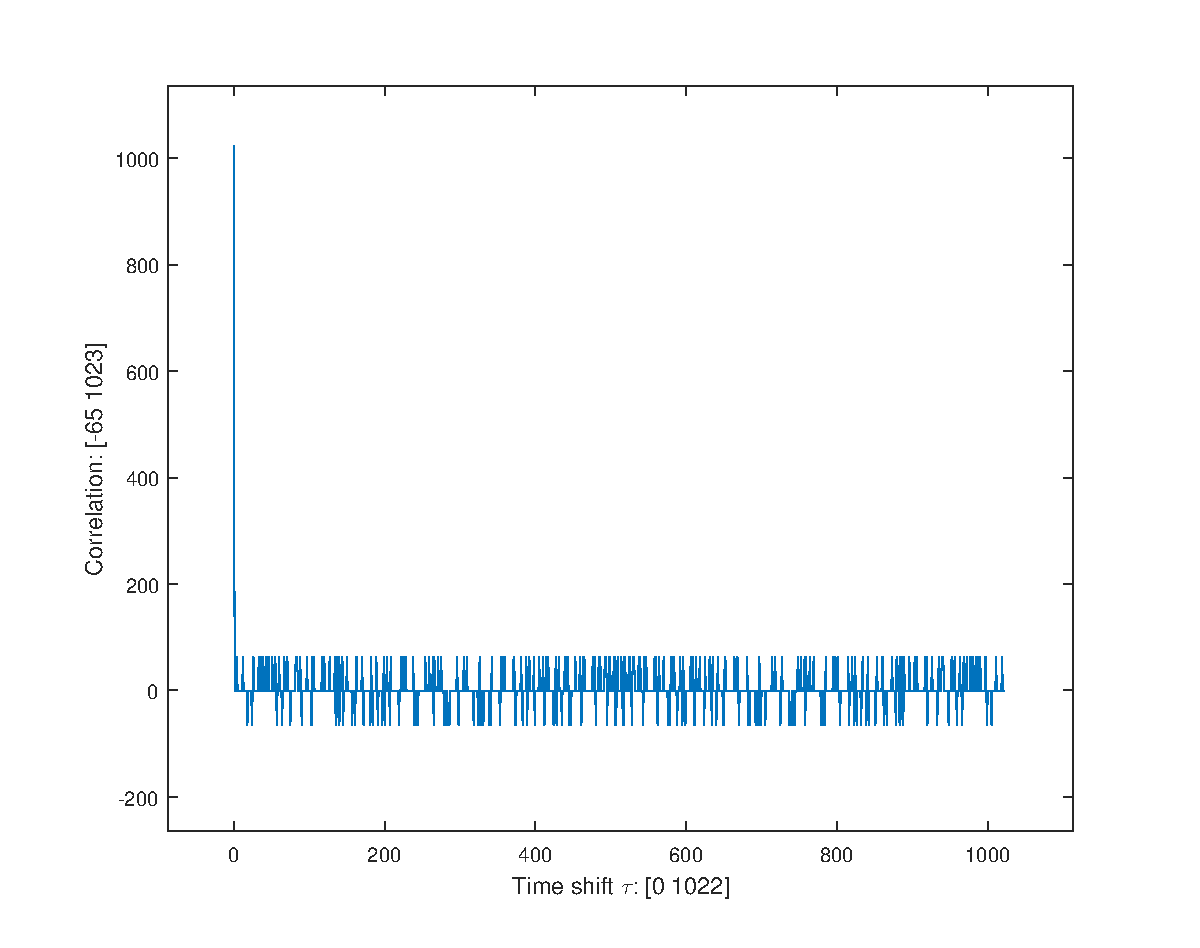
\includegraphics[width=\textwidth]{chapters/cdma-chapters/autocorr-gold.eps}
	\caption{Autocorrelation of one Gold sequence of length 1023.}
	\label{fig:autocorr-gold}
\end{figure}


\begin{figure}
	\centering
	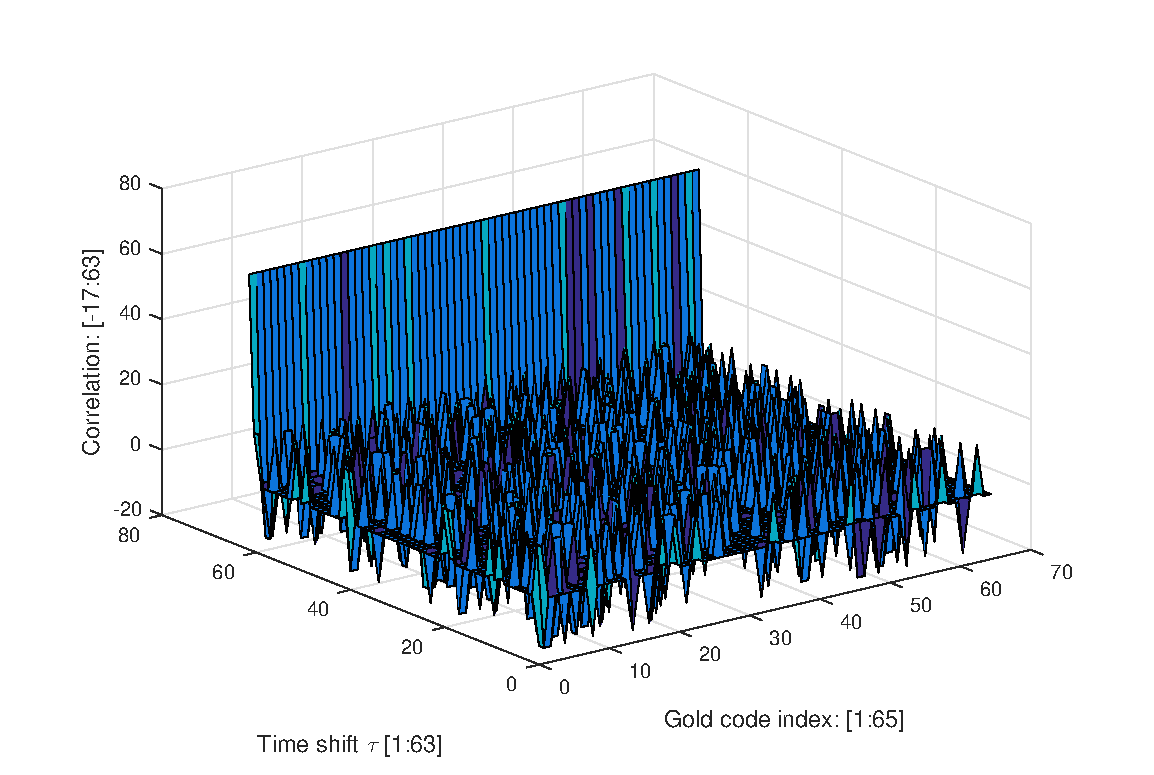
\includegraphics[width=\textwidth]{chapters/cdma-chapters/autocorr-gold-3d.eps}
	\caption{Autocorrelation of all Gold codes in the same set of length 63.}
	\label{fig:autocorr-gold-3d}
\end{figure}




The autocorrelation properties of Gold sequences are not as good as that of the PN sequences, as can be seen from \autoref{fig:autocorr-gold-3d}.
Apart from the original two PN sequences the autocorrelation values are not two-valued, but are four-valued.
See \autoref{eq:autocorr-gold} and \autoref{eq:gold-t(n)} for the autocorrelation properties of Gold sequences.

\begin{equation}
	\label{eq:autocorr-gold}
	R(\tau) = 
		\begin{cases}
			L    							& \quad \text{if } \tau = 0 \\
			\{ -t(n), \ -1, \ t(n) - 2  \} 	& \quad \text{if } \tau \neq 0 \\
		\end{cases}
\end{equation}

\begin{equation}
	\label{eq:gold-t(n)}
	t(n) = 
		\begin{cases}
			1 + 2^{\frac{n+1}{2}} & \quad \text{for odd } n \\
			1 + 2^{\frac{n+2}{2}} & \quad \text{for even } n \\
		\end{cases}
\end{equation}

See \autoref{eq:corsscorr-gold} and \autoref{eq:gold-t(n)} for the cross-correlation properties of Gold sequences \cite{mitra2008pseudo}.

\begin{equation}
	\label{eq:corsscorr-gold}
	R_{xy}(\tau) = 	\{ -t(n), -1, t(n) - 2  \} 
\end{equation}


From these equations it is clear to see that the absolute maximum cross-correlation is bounded by $t(n)$.

When $n$ is chosen to be odd, something can be said about the approximate frequency of occurrence of the cross-correlation values, see \autoref{tbl:freq-occurence-gold-cross-correlation} \cite{holmes2007spread}.

\begin{table}[h]
	\centering
	\begin{tabular}{ | l | l | }

		\hline
		$R_{xy}(\tau)$ 	& Frequency of occurrence	\\ \hline

		$-1$			& 0.5					 	\\ \hline
		$-t(n)$			& 0.25						\\ \hline
		$t(n) - 2$		& 0.25						\\ \hline

		

	\end{tabular}
	\caption{Table containing the approximate frequency of occurrence for all the cross-correlation values for $n$ odd.}
	\label{tbl:freq-occurence-gold-cross-correlation}
\end{table}

The Gold sequences posses good auto- and crosscorrelation, suitable for a-synchronous usage.
\todo{Also state that this is extra good, because the LEDs/transmitters cannot be synchronized ???}
Also the codes scale well.
With a LFSR of length $n$, the sequence length is $L = 2^n - 1$ and the number of sequences is $C = 2^n + 1$.

\todo{What information is really needed and which (like this table) is not necessary}










